\documentclass[UTF8]{ctexart}
\usepackage{ctex}
\usepackage{geometry}
\usepackage{enumitem}
\usepackage{indentfirst}
\usepackage{color}
\usepackage{fancyhdr}
\usepackage{amsmath}
\usepackage{graphicx}
\usepackage{amssymb}
\usepackage{tikz}
\usepackage{cases}
\usepackage{array}
\usepackage{pgfplots}
\usepackage{tkz-euclide}
\usepackage{mathrsfs}
% 设置纸张和页边距——A4
\geometry{papersize={21cm,29.7cm}}
\geometry{left=3.18cm,right=3.18cm,top=2.54cm,bottom=2.54cm}

% 一级标题靠左
\CTEXsetup[format={\Large\bfseries}]{section}

% 去除页眉
\pagestyle{plain}

%设置段间距
\addtolength{\parskip}{.4em}
%%设置行间距
%\usepackage{setspace}
%\setstretch{2.5}

% 开始文档内容
\begin{document}

\title{信号与系统课程笔记:Lecture 24:Z变换}
\author{授课教师:秦雨潇 \\
        笔记记录:曹时成}
\date{2023 年 12 月 1 日(第十三周,周五)}
\maketitle

\section{遗留问题:劳斯准则}
\qquad $a_ns^n+a_{n-1}s^{n-1}+a_{n-2}s^{n-2}+\cdots +a_{1}s+a_0=0$\par
判断该函数是否有负根?\par
有一个n+1行列的矩阵形式:\par
\begin{figure}[h]
    \centering         %使图片居中放置
    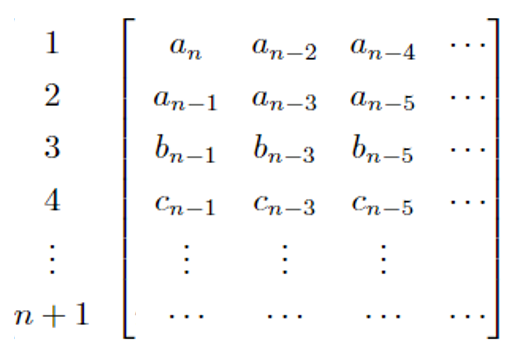
\includegraphics[scale=0.5]{1.png}
\end{figure}
其中:\par
\[b_{n-1}=-\frac{1}{a_{n-1}} \left[   
    \begin{matrix}
    a_{n} & a_{n-2} \\
    a_{n-1} & a_{n-3} \\
    \end{matrix}
     \right]  \]
\[b_{n-3}=-\frac{1}{a_{n-1}} \left[   
        \begin{matrix}
        a_{n} & a_{n-1} \\
        a_{n-1} & a_{n-5} \\
        \end{matrix}
         \right]  \]
\[c_{n-1}=-\frac{1}{b_{n-1}} \left[   
            \begin{matrix}
            a_{n-1} & a_{n-3} \\
            b_{n-1} & b_{n-3} \\
            \end{matrix}
             \right]  \]
\[c_{n-3}=-\frac{1}{b_{n-1}} \left[   
                \begin{matrix}
                a_{n-1} & a_{n-5} \\
                b_{n-1} & b_{n-5} \\
                \end{matrix}
                 \right]  \]
\qquad $\cdots $以此类推,求出矩阵最终形式.\par
\begin{figure}[h]
    \centering         %使图片居中放置
    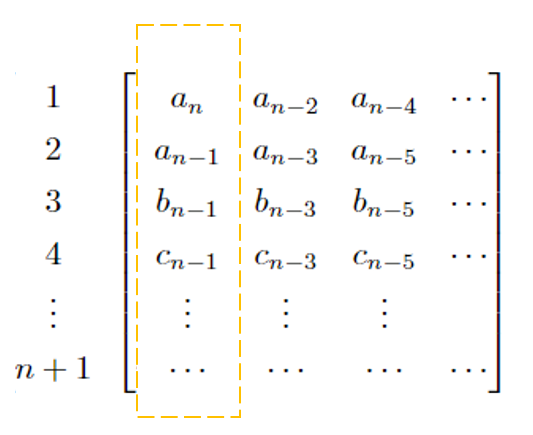
\includegraphics[scale=0.5]{2.png}
\end{figure}
如果矩阵第一列产生符号变化则有负根,对应系统不稳定.\par

\section{Z变换}
系统 \qquad 连续 \qquad  \qquad \qquad 离散 \par
时域 \qquad $f(t)\ast h(t)$ \qquad $f[k]\ast h[k],k\in \mathbb{Z}$  \par
频域 \qquad $F(w)H(w)$ \qquad DTFT \par
S域 \qquad $F(s)H(s)$ \qquad Z变换:$F(z)=\sum_{-\infty }^{+\infty} f[k]z^{-k} $ \par
信号的连续/离散域关系: \par
$F[k]=\sum_{-\infty }^{+\infty} f(t)\delta (t-nT_s),T_s=\frac{2\pi}{\Omega }  $  \par
\qquad $=\sum_{-\infty }^{+\infty} f(nT_s)\delta (t-nT_s), n\in \mathbb{Z} $  \par
\subsection{Discrete Time Fourier Transform}
连续信号FT:$F(\omega )=\int_{\mathbb{R} }f(t)e^{-jwt} \,dt $  \par
DTFT: $F(\omega )=\sum_{-\infty }^{+\infty} f[k]e^{-jwk},k\in \mathbb{Z},w\in \mathbb{R} $  \par
DTFT变换后也是连续频谱!\par
$F(\omega )=\int_{\mathbb{R} }f(t)e^{-jwt} \,dt $ (连续$\longrightarrow $ 离散) \par
$\int_{\mathbb{R} }\sum_{-\infty }^{+\infty} f(nT_s)\delta (t-nT_s)e^{-jwt} \,dt $ \par
$=\sum_{-\infty }^{+\infty} f(nT_s)\int_{\mathbb{R} }\delta (t-nT_s)e^{-jwt} \,dt $ \par
\begin{figure}[h]
    \centering         %使图片居中放置
    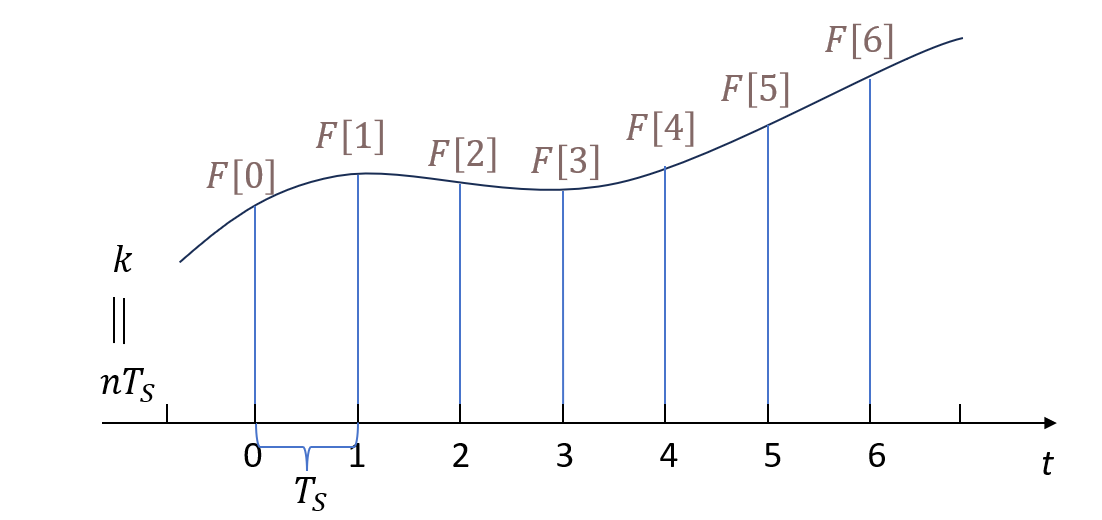
\includegraphics[scale=0.38]{3.png}
\end{figure}
$F(\omega )=\sum_{n=-\infty }^{+\infty} f(nT_s)e^{-jnT_sw}$ \par 
令$k=nT_s$ \par 
$F(\omega )=\sum_{n=-\infty }^{+\infty} f[k]e^{-jw}$ \par 
\subsection{从DTFT推导Z变换}
$F(z )=\sum_{n=-\infty }^{+\infty} f(nT_s)e^{-j(nT_s)w}$ \par 
\qquad $=\sum_{n=-\infty }^{+\infty} f(nT_s)re^{(jw)-nT_s}$ \par 
令 $z=re^{(jw)}$ \par 
\qquad $=\sum_{n=-\infty }^{+\infty} f(nT_s)z^{-nT_s}$ \par
令 $k=nT_s$ \par 
\qquad $=\sum_{n=-\infty }^{+\infty} f[k]z^{-k}$ \par
\subsection{从S域推导Z变换}
$f(t)\longleftrightarrow \sum_{-\infty }^{+\infty} f(nT_s)\delta (t-nT_s), n\in \mathbb{Z} $  \par
进行拉普拉斯变换:\par
$F(s)\longleftrightarrow  f(nT_s) \mathscr{L}\{\sum_{n=-\infty }^{+\infty}\delta (t-nT_s)\} $  \par
令$e^s=z$ \par
\qquad $=\sum_{n=-\infty }^{+\infty} f(nT_s)e^{s(nT_s)}$  \par
令 $k=nT_s$ \par 
\qquad $=\sum_{n=-\infty }^{+\infty} f[k]z^{-k}$  \par


\end{document}